\begin{figure*}[ht!] % or other placement options
\centering
%\begin{minipage}[b]{0.60\textwidth} % Adjust width as needed
\centering
\scalebox{.85}{
\begin{tabular}{lcccc}
\toprule
 & MSE \textsc{SP} ($\downarrow$) & $\rho$ \textsc{SP} ($\uparrow$) & MSE ET+SP ($\downarrow$) & $\rho$ ET+SP ($\uparrow$)\\
\midrule
Emp. mean & 0.01151 & N/A & 0.01250 & N/A  \\
\textsc{Linear} & 0.01637 & 0.23426 & 0.00655 & 0.64618 \\
MTGP & 0.00460 & 0.85829 & 0.00231 & 0.89911 \\
\textsc{BiMix}{\tiny{~\cite{bimix}}} & 0.00327 & 0.86051 & N/A  & N/A  \\
DML{\tiny{~\cite{dml}}} & 0.00296 & 0.91991 & 0.00116 & 0.89188 \\
GBM{\tiny{\textsc{RegMix}~\cite{regmix}}} & 0.00242 & 0.92256 & 0.00431 & 0.81442 \\
\midrule
MDE {\tiny{(ours)}} & 0.02809 & 0.91222 & 0.00391 & 0.88571 \\
GBM+MDE {\tiny{(ours)}} & 0.00140 & 0.94963 & 0.00089 & \textbf{0.95462} \\
\textsc{Linear}+MDE {\tiny{(ours)}} & \textbf{0.00050} & 0.97555 & \textbf{0.00048} & 0.95274 \\
MTGP+MDE {\tiny{(ours)}} & 0.00053 & \textbf{0.98383} & 0.00116 & 0.93469 \\
\bottomrule
\end{tabular}
}
%\end{center}
\captionsetup{type=table}
%\captionsetup{name=Table}
\caption{Mean squared error (MSE) and Spearman's rank correlation ($\rho$) on prediction of averaged loss over SlimPajama domains only (\textsc{SP}) and all (\textsc{ET+SP}) validation domains, using different regressors from prior work, and ones proposed in this work.   Regressors are fitted using 25 train mixtures (except MDE that uses only 7 train mixtures), and evaluated with 48 held-out mixtures. MDE features bring large improvements across regressors.}
\label{tab:regressors_sxs}
%\end{minipage} % \hfill % Adds horizontal space between minipages
%\hfill
% \begin{minipage}[b][][b]{0.31\textwidth}

\end{figure*}

\begin{figure}[]
\centering
       
 
 \scalebox{.7}{

  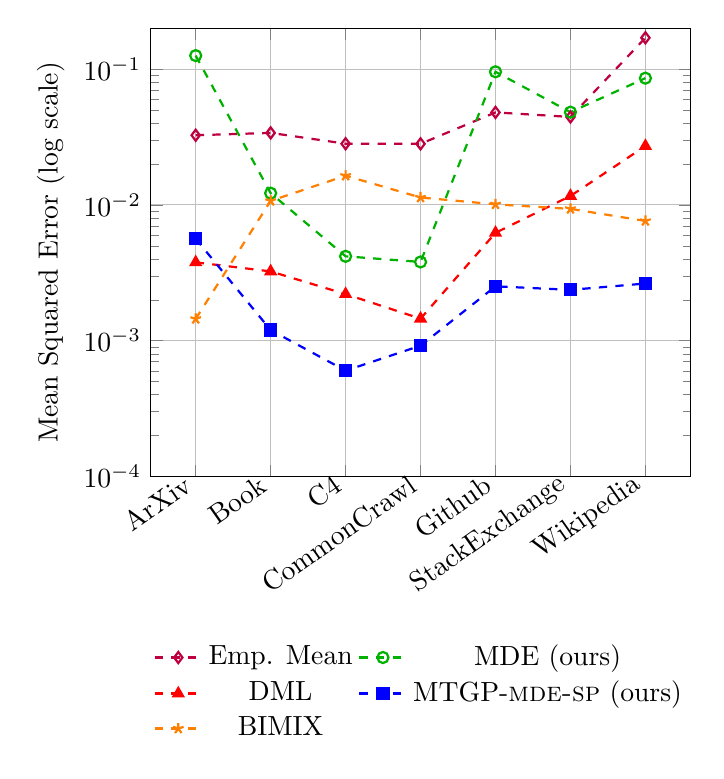
\begin{tikzpicture}
    \begin{axis}[
      ylabel={Mean Squared Error (log scale)},
      ymode=log,
      symbolic x coords={ArXiv,Book,C4,CommonCrawl,Github,StackExchange,Wikipedia},
      xtick=data,
      ymin=0.0001,
      ymax=0.2,
      grid=major,
      legend style={at={(0.5,-0.35)}, anchor=north, legend columns=2, draw=none}, % Modified to 2 columns
      x tick label style={rotate=35, anchor=east},
      mark options={solid},
    %   width=0.95\textwidth, % Make the plot wider
    %   height=0.6\textwidth, % Adjust the height to keep aspect ratio
    ]

      % emp. mean
      \addplot[dashed, mark=diamond, color=purple, thick] coordinates {
        (ArXiv,0.03258848761214498) 
        (Book,0.033901799466678983) 
        (C4,0.028237080166221618) 
        (CommonCrawl,0.028170427516745984) 
        (Github,0.04799648997394152) 
        (StackExchange,0.04444072752490156) 
        (Wikipedia,0.16998068744909084)
      };
      \addlegendentry{Emp. Mean}

      % mde
      \addplot[dashed, mark=o, color=green!70!black, thick] coordinates { % Darker green
        (ArXiv,0.12569990165231987) 
        (Book,0.012200067712023305) 
        (C4,0.004183705236557251) 
        (CommonCrawl,0.0038020182635709896) 
        (Github,0.09553608975123355) 
        (StackExchange,0.048190113535861154) 
        (Wikipedia,0.08576905332796389)
      };
      \addlegendentry{MDE (ours)}

      % dml
      \addplot[dashed, mark=triangle*, color=red, thick] coordinates {
        (ArXiv,0.0037785496210790935) 
        (Book,0.0032396400943874803) 
        (C4,0.0022037963338795985) 
        (CommonCrawl,0.0014545846122193365) 
        (Github,0.006231348171967968) 
        (StackExchange,0.01163995357956378) 
        (Wikipedia,0.027135803524510626)
      };
      \addlegendentry{DML}

      % mtgp_mde
      \addplot[dashed, mark=square*, color=blue, thick] coordinates {
        (ArXiv,0.005638437945592803) 
        (Book,0.001197677572446236) 
        (C4,0.0006021703300710033) 
        (CommonCrawl,0.0009188736749797932) 
        (Github,0.0025156553673455454) 
        (StackExchange,0.002369188450940196) 
        (Wikipedia,0.0026375685939519487)
      };
      \addlegendentry{MTGP-\textsc{mde-sp} (ours)}

      % bimix
      \addplot[dashed, mark=star, color=orange, thick] coordinates {
        (ArXiv,0.0014483220708567256) 
        (Book,0.010711812127249159) 
        (C4,0.01641659212707495) 
        (CommonCrawl,0.01133554534292917) 
        (Github,0.010100280035751018) 
        (StackExchange,0.00934835484835737) 
        (Wikipedia,0.0076224179394367726)
      };
      \addlegendentry{BIMIX}

    \end{axis}
  \end{tikzpicture}
  }
  \caption{Per-domain mean loss squared error for SlimPajama validation domains.}
  \label{fig:280M_to_280M_train_only_loss_error_per_domain_sxs}
\end{figure}





